\documentclass[12pt]{article}

\usepackage{fullpage}
\usepackage[spanish]{babel}
\usepackage{amsfonts} %for double trace letters
\usepackage{amssymb}
\usepackage{amsmath} %for special/unusual mathematical characters
\usepackage{eufrak} %for gothic letters
\usepackage{graphicx} %Image includer package
\graphicspath{{Images/}} %Image directory
\usepackage{xcolor}
\usepackage{esint} % for simple counter-clockwise directed contour integral symbol

% For index
\usepackage[utf8]{inputenc}
\usepackage{imakeidx}
\usepackage{hyperref}% for hyperlinked index
\makeindex

% For table of contents with links to section
\usepackage{hyperref}
\hypersetup{
    colorlinks=true, %set true if you want colored links
    linktoc=all,     %set to all if you want both sections and subsections linked
    linkcolor=black,  %choose some color if you want links to stand out
}

\usepackage{multicol} %For writing text in columns
\setlength{\columnsep}{1cm} %Defines separation of columns

\usepackage{tcolorbox} %for boxes that enclose text
\usepackage{color}
\definecolor{myblue}{rgb}{.8, .8, 1}

\usepackage{empheq}

%for green eq box
%\definecolor{lightgreen}{HTML}{90EE90}
%\newcommand{\boxedeq}[2]{\begin{empheq}[box=\colorbox{lightgreen}]{align}\label{#1}#2\end{empheq}}

%for blue eq box
\newlength\mytemplen
\newsavebox\mytempbox

\makeatletter
\newcommand\mybluebox{%
    \@ifnextchar[%]
       {\@mybluebox}%
       {\@mybluebox[0pt]}}

\def\@mybluebox[#1]{%
    \@ifnextchar[%]
       {\@@mybluebox[#1]}%
       {\@@mybluebox[#1][0pt]}}

\def\@@mybluebox[#1][#2]#3{
    \sbox\mytempbox{#3}%
    \mytemplen\ht\mytempbox
    \advance\mytemplen #1\relax
    \ht\mytempbox\mytemplen
    \mytemplen\dp\mytempbox
    \advance\mytemplen #2\relax
    \dp\mytempbox\mytemplen
    \colorbox{myblue}{\hspace{1em}\usebox{\mytempbox}\hspace{1em}}}

% For arrow comment
\usepackage{tikz}
\usetikzlibrary{tikzmark,arrows,calc}
\newcommand\sidecomment[5][0.3,0.1]%
  {\begin{tikzpicture}[remember picture,overlay]
   \draw[-stealth',thick]
     ($({pic cs:#4}|-{pic cs:#2})+(#1)$)
     .. controls +(1,0) and +(1,0) ..
     node[right,align=left]{#5}
     ($({pic cs:#4}|-{pic cs:#3})+(#1)$);
   \end{tikzpicture}%
  }

% for theorems
\usepackage{amsthm}
 
\theoremstyle{definition}
\newtheorem{definition}{Definici\'on}[section]

\theoremstyle{theorem}
\newtheorem{theorem}{Teorema}[section]

\theoremstyle{corolary}
\newtheorem{corolary}{Corolario}[section]

\theoremstyle{method}
\newtheorem{method}{Regla}

\DeclareMathOperator{\Arg}{Arg}
\DeclareMathOperator{\Log}{Log}
\DeclareMathOperator{\sen}{sen}
\DeclareMathOperator{\senh}{senh}
\DeclareMathOperator{\tg}{tg}
\DeclareMathOperator{\ctg}{ctg}
\DeclareMathOperator{\tgh}{tgh}
\DeclareMathOperator{\ctgh}{ctgh}
\DeclareMathOperator{\sech}{sech}
\DeclareMathOperator{\csch}{csch}
%\DeclareMathOperator{\Res}{Res}
\DeclareMathOperator*{\Res}{Res}

\begin{document}
	\title{Sucesiones y series de n\'umeros complejos}
	\author{Breggia, Bruno M.}
	\date{}
	\maketitle

\begin{center}
	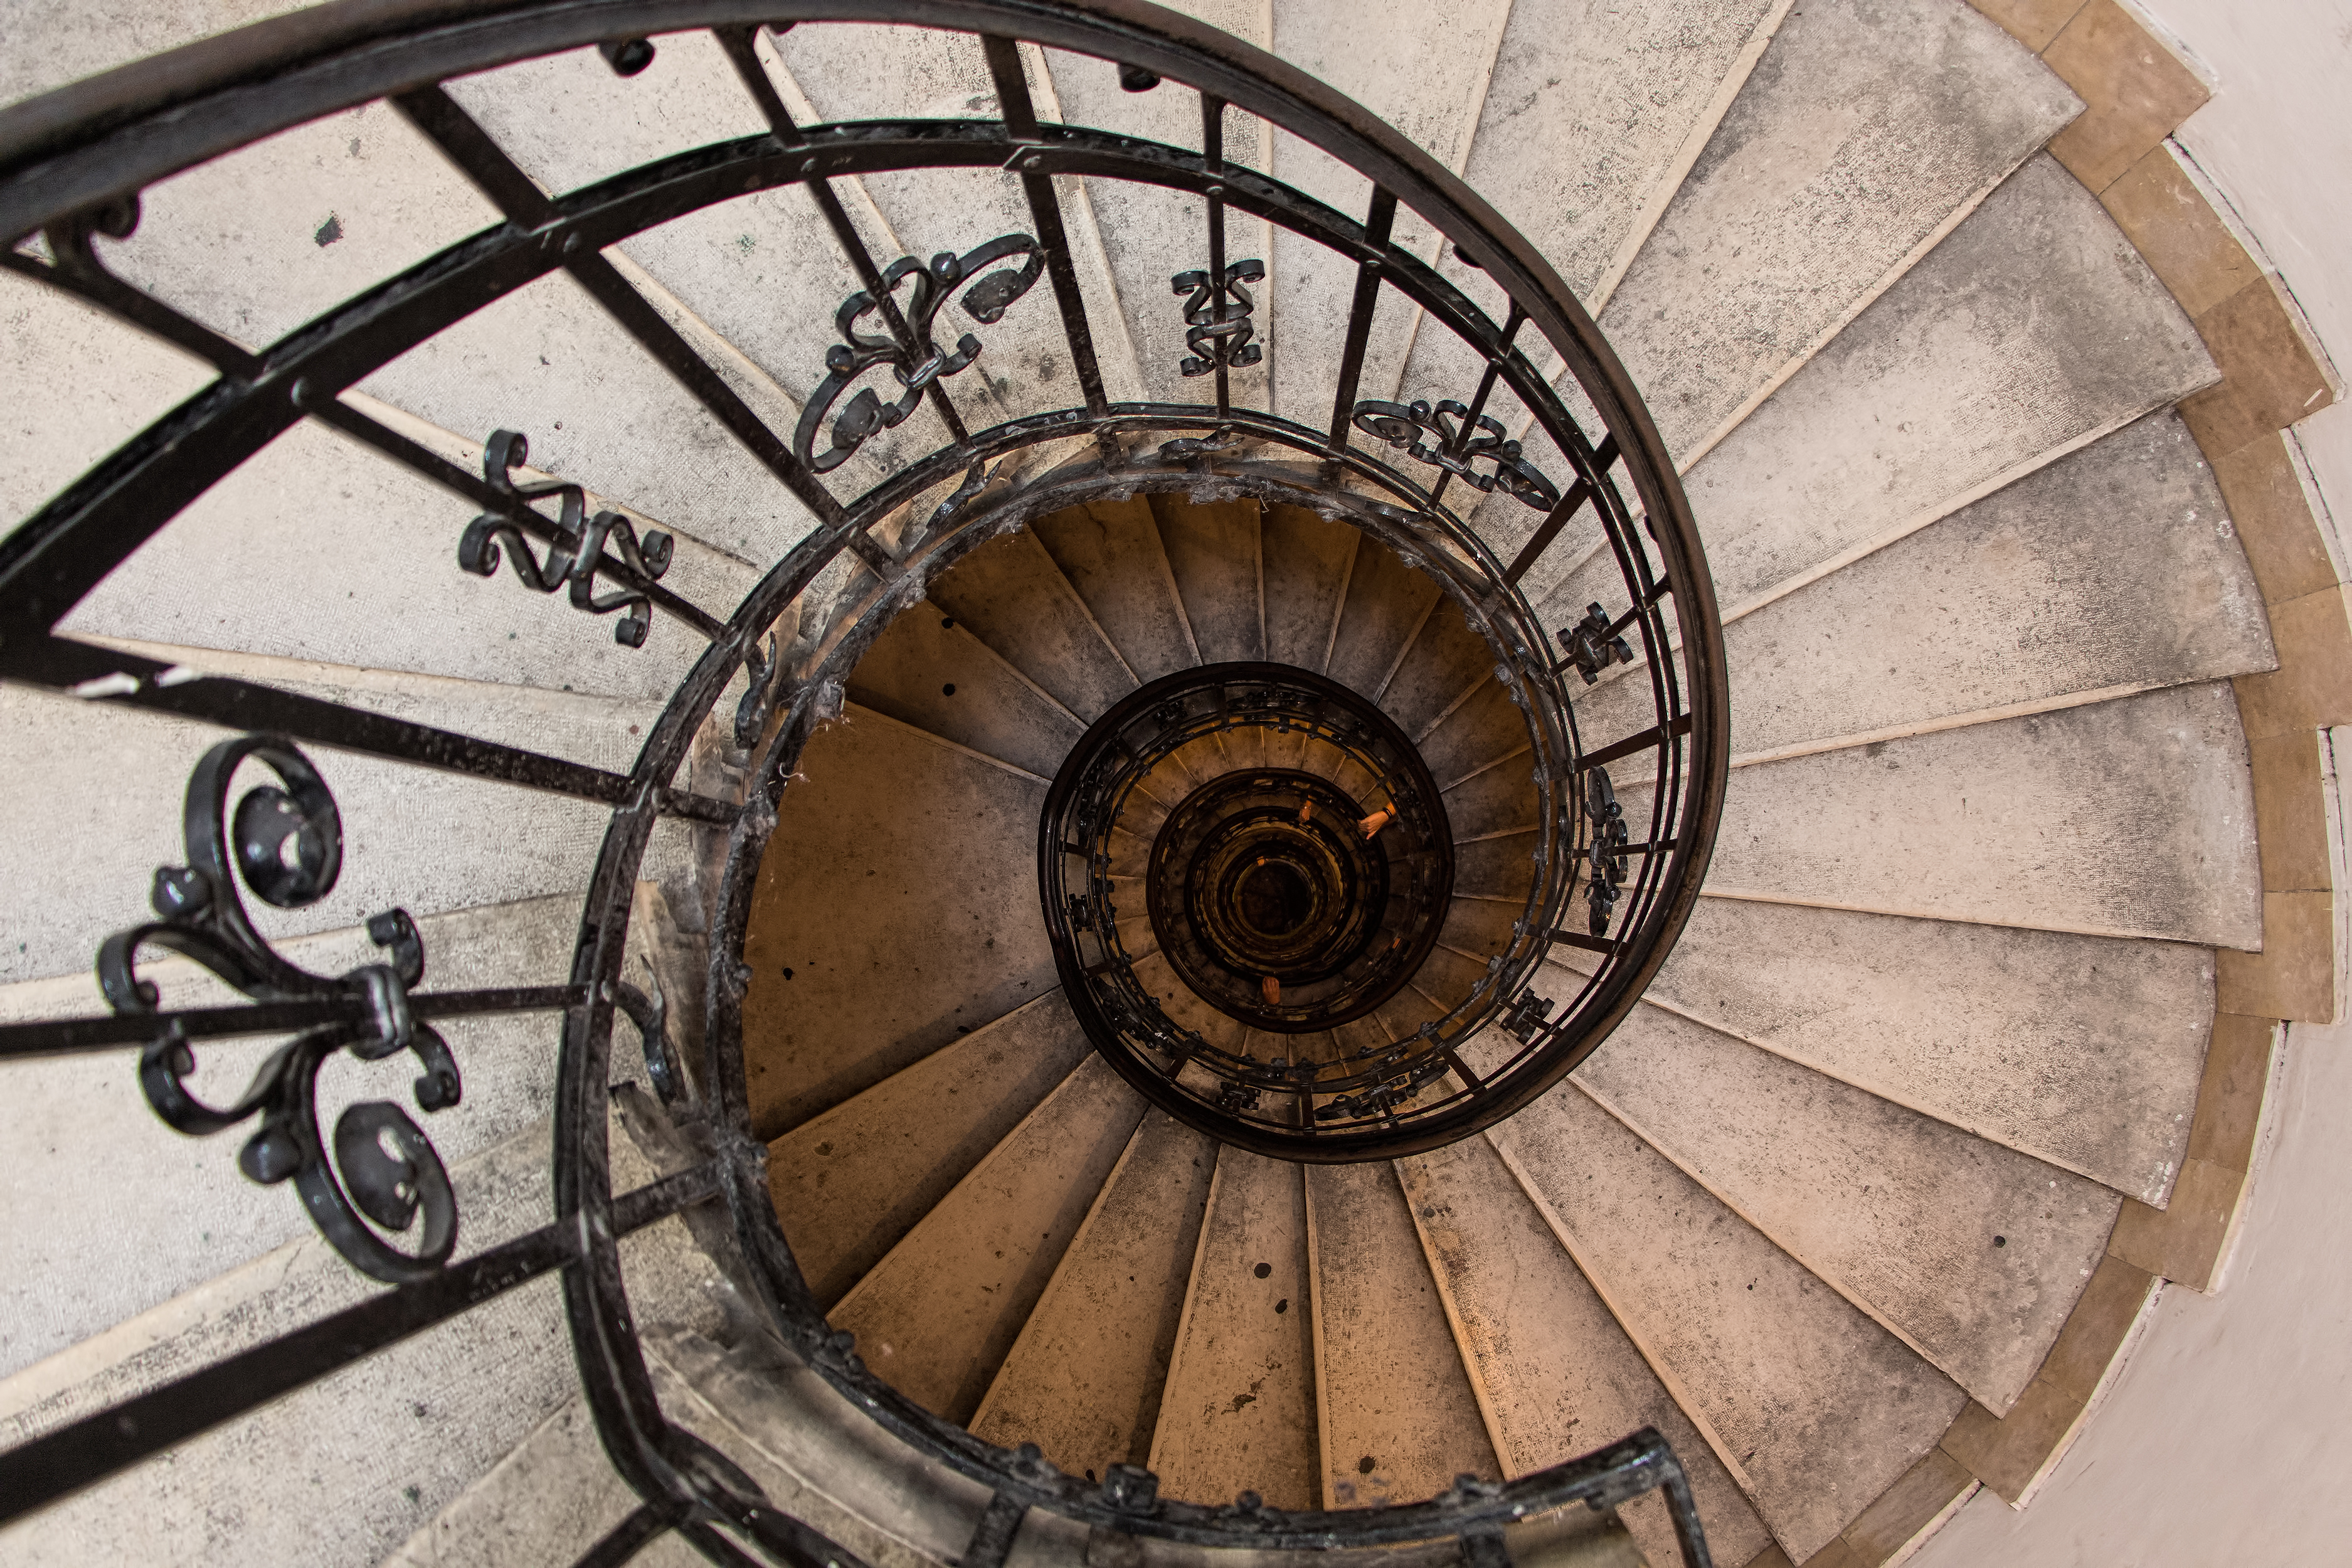
\includegraphics[scale=0.45]{staircase.jpg}
\end{center}

Qui\'en alguna vez no se durmi\'o contando ovejas... Claro qued\'o desde que se introdujeron los n\'umeros complejos que los n\'umeros no son todos para contar. El conjunto $\mathbb{C}$ no es un conjunto ordenado, pero no por ello nos vemos incapacitados de crear nuestras propias sucesiones de complejos. Y cuando hablo de sucesiones, hablo de sucesiones infinitas, como debe ser. Pero en vez de corresponderse con puntos en la recta num\'erica, aqu\'i las sucesiones ser\'an... puntos desparramados en el plano. Una cosa les anticipar\'e: trabajar con sucesiones y series implica domar el infinito, y para ello volveremos a nuestro olvidado amigo el plano complejo extendido $\mathbb{C}^{\infty}$, es decir, encarnaremos al infinito mismo en un punto... en un simple punto como cualquier otro... un mortal como los dem\'as. !`In\'iciese este cap\'itulo o no se acabar\'a jam\'as!

\pagebreak
\tableofcontents
\pagebreak

\section{Sucesiones de n\'umeros complejos}
Todos conocemos las sucesiones... de n\'umeros reales. Pero a ser verdad, una sucesi\'on de n\'umeros complejos es una sucesi\'on que, sorpresa, posee n\'umeros complejos. Abstraer la idea de sucesi\'on no es en absoluto complicado. Sin embargo, la definici\'on formal nunca debe faltar:\\

\colorbox{violet!40!white!80}{\parbox{\linewidth}{
\theoremstyle{definition}
\begin{definition}{Sucesiones de n\'umeros complejos}

Una \textbf{sucesi\'on} de n\'umeros complejos es una relaci\'on que a cada $n\in \mathbb{N}$ se le asigna un $z_n \in \mathbb{C}$, es decir: $$n\in \mathbb{N} \rightarrow z_n\in \mathbb{C}$$

\end{definition}}}
\linebreak
\linebreak

%\begin{multicols}{2}
Hay dos maneras de anotar una sucesi\'on:
\begin{itemize}
	\item \textbf{Por comprensi\'on}: consiste en denotar el t\'ermino general $z_n$ entre llaves $$\{z_n\}$$
	\item \textbf{Por extensi\'on}: consiste en nombrar uno por uno los elementos (preferiblemente los primeros) de la sucesi\'on $$z_1, z_2, z_3, ... ,z_n, ...$$
\end{itemize}

\begin{center}
	\includegraphics[scale=0.2]{hormigas2.jpg}
\end{center}
%\end{multicols}

Vamos a repasar y pasar en limpio algunos conceptos aplicados a las sucesiones de n\'umeros reales, pero aplicados a las de complejos. Primero y principal: \textbf{convergencia}.\\

\colorbox{violet!40!white!80}{\parbox{\linewidth}{
\theoremstyle{definition}
\begin{definition}{Convergencia}

Una sucesi\'on $\{z_n\}$ se dice ser \textbf{convergente} a un valor $z \in \mathbb{C}$ si y s\'olo si dado un $\varepsilon \in \mathbb{R}^+$ existe un $\delta \in \mathbb{N}$ tal que $$|z_n-z|<\varepsilon$$ para todo $n>\delta$.\\
Si esto se cumple, diremos entonces que la sucesi\'on posee l\'imite, y lo denotaremos como: $$\lim\limits_{n\rightarrow \infty} z_n = z$$
Si una sucesi\'on no es convergente, se dir\'a que es \textbf{divergente}.

\end{definition}}}
\linebreak
\linebreak

\begin{center}
	\includegraphics[scale=0.8]{limite.png}
\end{center}

De manera an\'aloga a la de l\'imites de funciones de variable compleja, es demostrable (y tambi\'en bastante intuitivo) que el l\'imite de una sucesi\'on, si existe, es \'unico.\\

\colorbox{red!40!white!80}{\parbox{\linewidth}{
\theoremstyle{theorem}
\begin{theorem} {Unicidad del l\'imite}

Si una sucesi\'on posee l\'imite, entonces su l\'imite es \'unico.
\end{theorem}}}
\linebreak
\linebreak

El pr\'oximo teorema nos vincula el l\'imite de sucesiones de n\'umeros complejos con l\'imites de n\'umeros reales. Dif\'icil no entenderlo.\\

\colorbox{red!40!white!80}{\parbox{\linewidth}{
\theoremstyle{theorem}
\begin{theorem} {L\'imite de una sucesi\'on de complejos}

Sea $\{z_n\}$ una sucesi\'on de n\'umeros complejos y sea $z\in \mathbb{C}$, tal que $z_n = x_n + i\ y_n\ \	land\ z=x+i\ y$.\\
Entonces: $$\lim\limits_{n\rightarrow \infty} z_n = z \Leftrightarrow \lim\limits_{n\rightarrow \infty}x_n = x\:\land\:\lim\limits_{n\rightarrow \infty}y_n = y$$
\end{theorem}}}
\linebreak
\linebreak

De esta manera, el estudio de sucesiones de n\'umeros complejos se reduce al estudio de dos sucesiones de n\'umeros reales. Y ya sabemos c\'omo operar con ellas.

\section{Series de n\'umeros complejos}
Procederemos de igual manera a dar definiciones rigurosas de lo que son las series de n\'umeros complejos.\\

\colorbox{violet!40!white!80}{\parbox{\linewidth}{
\theoremstyle{definition}
\begin{definition}{Serie de n\'umeros complejos}

Se denomina \textbf{serie} de n\'umeros complejos $z_1+z_2+z_3+...+z_n+...$
a la sucesi\'on de sumas parciales $\{S_N\}$ siendo $$S_N = \sum\limits_{k=1}^N z_k$$ con $n, k \in \mathbb{N}$ y $z_k \in \mathbb{C}$.

\end{definition}}}
\linebreak
\linebreak

\begin{center}
	\includegraphics[scale=1.3]{series.jpg}
\end{center}

La serie se defini\'o como una \textbf{sucesi\'on}, por lo que la misma puede ser o no convergente.\\

\colorbox{violet!40!white!80}{\parbox{\linewidth}{
\theoremstyle{definition}
\begin{definition}{Serie convergente}

Una serie de n\'umeros complejos $z_1+z_2+z_3+...+z_n+...$
se dice \textbf{convergente} si y s\'olo si la sucesi\'on de sumas parciales $\{S_N\}$ es convergente a alg\'un valor $S \in \mathbb{C}$.\\
En caso contrario la serie ser\'a \textbf{divergente}.

\end{definition}}}
\linebreak

\begin{center}
	\includegraphics[scale=0.5]{suma_parcial.jpg}
\end{center}

Pero como el $n$-\'esimo t\'ermino de una serie representa la suma parcial de los $n$ primeros t\'erminos de alguna otra sucesi\'on $\{z_n\}$, entonces si la serie converge, esto quiere decir que encontramos el l\'imite para la suma de todos los t\'erminos de la sucesi\'on $\{z_n\}$. Por esto mismo es que viene a colaci\'on la siguiente definici\'on:\\

\colorbox{violet!40!white!80}{\parbox{\linewidth}{
\theoremstyle{definition}
\begin{definition}{Suma de la serie convergente}

En caso de que la sucesi\'on de sumas parciales $\{S_N\}$ sea convergente a $S \in \mathbb{C}$, se dice que $S$ es la \textbf{suma de la serie}, y se indica, por comprensi\'on: $$S=\sum\limits_{n=1}^{\infty}z_n$$
\'o por extensi\'on: $$z_1+z_2+z_3+...+z_n+...$$
\end{definition}}}
\linebreak
\linebreak

%\begin{center}
%	\includegraphics[scale=1]{loading.jpg}
%\end{center}

Ahora, el teorema que nos vincula las series de n\'umero complejos con series de n\'umeros reales:\\

\colorbox{red!40!white!80}{\parbox{\linewidth}{
\theoremstyle{theorem}
\begin{theorem} {Convergencia de series de n\'umeros complejos}

Una serie de n\'umeros complejos se dice convegrnete si y s\'olo si la serie de la parte real y la serie de la parte imaginaria son ambas convergentes en $\mathbb{R}$.\\
Simb\'olicamente, sean $z_n,S \in \mathbb{C}\ /\ z_n = x_n + i\ y_n\:\land\:S = X + i Y$. Entonces: $$\sum\limits_{n=1}^{\infty}z_n=S\ \Leftrightarrow\ \sum\limits_{n=1}^{\infty}x_n = X\:\land\:\sum\limits_{n=1}^{\infty}y_n=Y$$
\end{theorem}}}
\linebreak
\linebreak

Esto nos trae como consecuencia el siguiente corolario, que presentar\'a la manera que utilizaremos de ahora en adelante para determinar la convergencia de series de n\'umeros complejos.\\

\colorbox{pink!40!white!80}{\parbox{\linewidth}{
\theoremstyle{theorem}
\begin{corolary} {Condici\'on de convergencia de series}

Una serie de n\'umeros complejos converge a $S$ si y s\'olo si la sucesi\'on de los restos $\{\rho_N\}$, definida con $\rho_N=S - S_N,$ converge a cero.\\
Es decir, si $$\lim\limits_{N\rightarrow \infty}\rho_N=\lim\limits_{N\rightarrow \infty}(S-S_N)=0$$
\end{corolary}}}
\linebreak
\linebreak

%\colorbox{violet!40!white!80}{\parbox{\linewidth}{
%\theoremstyle{definition}
%\begin{definition}{Convergencia de la sucesi\'on de los restos}

%La sucesi\'on $\{\ \rho_N \}$, con $\rho_N = S_N - S$, converge a $0$, es decir $\lim\limits_{N\to \infty}\rho_N=0$, si y s\'olo si dado un $\varepsilon \in \mathbb{R}^+$ existe un $M \in \mathbb{N}$ tal que: $$|\rho_N| = |S_N - S|<\varepsilon$$
%para todo $N > M$.
%\end{definition}}}
%\linebreak
%\linebreak


\section{Series de funciones complejas}
Ahora lleg\'o el momento de estudiar \textit{series de funciones complejas}. Es decir, una serie formada por las sumas parciales de una sucesi\'on que involucra una funci\'on de variable compleja en su t\'ermino general. En fin, el resultado es una funci\'on con varios t\'erminos, y mientras m\'as t\'erminos se consideren, mayor la precisi\'on del resultado.

Estudiaremos primero la serie m\'as com\'un, y \'util, que se nos presentar\'a de ahora en adelante...\\


\colorbox{yellow!40!white!80}{\parbox{\linewidth}{
\theoremstyle{definition}
\begin{definition}{Series de Potencias}

Las \textbf{series de potencias} son de la forma $$\sum\limits_{n=0}^{\infty}a_n(z-z_0)^n$$ donde $a_n, z_0\in \mathbb{C}$ y $z$ es cualquier punto de una regi\'on predeterminada en el plano complejo que contenga $z_0$.

\end{definition}}}
\linebreak
\linebreak

Con esta presentaci\'on oficial de lo que es una serie de potencias de n\'umeros complejos, podemos expresar su desarrollo como sigue: $$\sum\limits_{n=0}^{\infty}a_n(z-z_0)^n = a_0 + a_1(z-z_0)+a_2(z-z_0)^2+...+a_n(z-z_0)^n+...$$

Para el caso particular de que $a_n = 1$ y $z_0=0$, tenemos lo que denominamos \textbf{serie geom\'etrica}, la cual denotamos como $$\sum\limits_{n=0}^{\infty}z_n = 1+z+z^2+z^3+...+z^n+...$$

La \textbf{suma parcial} de la serie geom\'etrica hasta sus $N$ primeros t\'erminos (siempre que $z\neq 1$) viene dada por: $$S_N = \sum\limits_{n=0}^{N-1}z_n = \frac{1-z^N}{1-z}$$

Por otro lado, tenemos que si $|z|<1$, entonces la serie geom\'etrica es convergente, y la \textbf{suma de la serie} tiene curiosamente la forma: $$S = \sum\limits_{n=0}^{N-1}z_n = \frac{1}{1-z}$$

La serie goem\'etrica es efectivamente convergente porque el l\'imite de la \textbf{sucesi\'on de los restos} $\rho_N(z)$ tiende a cero conforme $N$ tiende a infinito. La expresi\'on para tal sucesi\'on (para el $N$-\'esimo t\'ermino) viene dada por: $$\rho_N(z)=\frac{z^N}{1-z}$$

Ahora, ustedes dir\'an: la expresi\'on para $\rho_N(z)$ claramente no se vuelve nada peque\~na conforme $N$ tienda a infinito. Si esto es lo que est\'an pensando, resuelvan el l\'imite. H\'aganlo e impongan condiciones para que tal l\'imite sea cero. Pues peque\~no detalle el que complejos $z\ /\ |z|<1$, al elevarlos a potencias positivas, su m\'odulo decrece, y con ello dicho l\'imite ser\'a cero.\\

Ahora, se vienen dos de las obras maestras del c\'alculo complejo basado en series...\\

\colorbox{blue!40!white!80}{\parbox{\linewidth}{
\theoremstyle{theorem}
\begin{theorem} {Teorema de Taylor}

Sea $f(z)$ una funci\'on anal\'itica en un disco abierto $\mathcal{D} \subset \mathbb{C}: |z-z_0|<R_0$. Entonces $\forall z\in \mathcal{D}$, $f(z)$ admite representaci\'on en \textbf{serie de Taylor}.
$$f(z)=\sum\limits_{n=0}^{\infty}a_n(z-z_0)^n\ ,\qquad |z-z_0|<R_0$$
en donde $$a_n=\frac{f^{(n)}(z_0)}{n!}, \qquad n\in \mathbb{N}$$
\end{theorem}}}
\linebreak
\linebreak

Esta obra maestra nos permite representar una funci\'on $f(z)$ mediante una serie de potencias centrada en $z_0$ siempre que lo hagamos dentro de una regi\'on en la cual $f(z)$ sea anal\'itica.

\begin{center}
	\includegraphics[scale=0.8]{taylor_reg.png}
\end{center}

Sin embargo, ?`qu\'e sucede si queremos centrarla en puntos en donde $f(z)$ no es anal\'itica, o de manera gen\'erica, si la regi\'on que consideramos contiene puntos en los cuales $f(z)$ no es anal\'itica? Para ello viene Laurent a salvarnos...\\

\colorbox{blue!40!white!80}{\parbox{\linewidth}{
\theoremstyle{theorem}
\begin{theorem} {Teorema de Laurent}

Sea $f(z)$ una funci\'on anal\'itica en un anillo $\mathcal{D} \subset \mathbb{C}: R_1<|z-z_0|<R_2$. Sea $\mathcal{C}$ un contorno cerrado simple orientado positivamente centrado en $z_0$, con $\mathcal{C}\subset \mathcal{D}$.\\
Entonces $\forall z\in \mathcal{D}$, $f(z)$ admite representaci\'on en \textbf{serie de Laurent}.
$$f(z)=\sum\limits_{n=0}^{\infty}a_n(z-z_0)^n+\sum\limits_{n=1}^{\infty}\frac{b_n}{(z-z_0)^n}\ ,\qquad R_1<|z-z_0|<R_2$$
en donde $$a_n=\frac{1}{2\pi i} \oint\limits_{\mathcal{C}}\frac{f(z)}{(z-z_0)^{n+1}} dz \qquad n\in \mathbb{N}_0$$
$$b_n=\frac{1}{2\pi i} \oint\limits_{\mathcal{C}}\frac{f(z)}{(z-z_0)^{-n+1}} dz \qquad n\in \mathbb{N}$$

\end{theorem}}}
\linebreak
\linebreak

Una expresi\'on alternativa para la \textbf{serie de Laurent} viene dada por:
$$f(z)=\sum\limits_{n=-\infty}^{\infty}c_n(z-z_0)^n\ ,\qquad R_1<|z-z_0|<R_2$$
...con los coeficientes $c_n$ determinados de la siguiente manera: $$c_n = \frac{1}{2\pi i}\oint\limits_{\mathcal{C}}\frac{f(z)}{(z-z_0)^{n+1}}\ dz \qquad n\in \mathbb{Z}$$

\begin{center}
	\includegraphics[scale=0.6]{anillo.png}
\end{center}

Claramente con Laurent podemos representar funciones $f(z)$ como series de potencias (positivas \textit{y} negativas) en donde la de Taylor no pod\'ia. A esto lo logramos esquivando, o evitando mejor dicho, a los puntos en donde la funci\'on no es anal\'itica. Pareciese ser que para aproximarse mejor al resultado en casos en que tengamos estos tipos de puntos la soluci\'on es concebir \textit{tambi\'en} infinitos t\'erminos de potencias decrecientes tanto como de potencias crecientes.

Por esto mismo la serie de Laurent pareciese ser m\'as potente. Barre rincones donde la de Taylor no llega. Notaremos la practicidad de la serie de Laurent a partir de estos casos particulares:
\begin{itemize}
	\item Cuando $R_1=0$, y el anillo se convierte en un entorno reducido dado por $\mathcal{D}: 0<|z-z_0|<R_2$
	\item Cuando $z_0=0\ \land\ R_2=\infty$, en donde tendr\'iamos lo que denominamos un entorno centrado en infinito dado por $\mathcal{D}:R_1<|z|<\infty$
\end{itemize}

\subsection{Serie de Laurent: $R_1=0$}
Sea $f(z)$ una funci\'on anal\'itica en $\mathcal{D} \subset \mathbb{C}:0<|z-z_0|<R$ donde $z_0$ es una \textbf{singularidad aislada} de $f(z)$. Entonces $f(z)$ puede representarse por una serie de Laurent:
$$f(z)=\sum\limits_{n=0}^{\infty}a_n(z-z_0)^n+{\color{blue}\sum\limits_{n=0}^{\infty}\frac{b_n}{(z-z_0)^n}}\ ,\qquad 0<|z-z_0|<R$$
en donde la sumatoria de t\'erminos con exponente negativo se denomina \textbf{parte principal} de $f$ en $z_0$: $$\color{blue}\sum\limits_{n=0}^{\infty}\frac{b_n}{(z-z_0)^n} = \frac{b_1}{(z-z_0)}+\frac{b_2}{(z-z_0)^2}+...+\frac{b_n}{(z-z_0)^n}+...$$

\begin{center}
	\includegraphics[scale=0.6]{entorno_red.png}
\end{center}

Cuando este caso particular se d\'e, podremos clasificar a la singularidad aislada en cuesti\'on en tres tipos: como \textbf{removible}, \textbf{polo de orden $m$}, o \textbf{esencial}.

\colorbox{yellow!40!white!80}{\parbox{\linewidth}{
\theoremstyle{definition}
\begin{definition}{Singularidad removible o evitable}

En $z_0$ existe una \textbf{singularidad removible} o \textbf{evitable} de $f(z)$ si se cumple:
\begin{itemize}
	\item $z_0$ es una singularidad aislada de $f(z)$
	\item El desarrollo en serie de Laurent de $f(z)$ centrado en $z_0$ con $R_1=0$ tiene parte principal nula. Es decir, los coeficientes $b_n$ son todos cero $$b_1=b_2=b_3=...=b_n=...=0$$
\end{itemize}
\end{definition}}}
\linebreak
\linebreak

Como consecuencia, se tiene que si $z_0$ es una singularidad removible, y se centra en \'el un desarrollo en serie de Laurent con $R_1=0$, tenemos que $$f(z)=\sum\limits_{n=0}^{\infty}a_n(z-z_0)^n\ , \qquad 0<|z-z_0|<R_2$$
Tal expresi\'on es similar a una serie de Taylor, pero v\'alida en un entorno reducido (que no incluye $z_0$), y en donde se cumple el siguiente l\'imite: $$\lim\limits_{z\rightarrow z_0}f(z)=a_0$$

\colorbox{yellow!40!white!80}{\parbox{\linewidth}{
\theoremstyle{definition}
\begin{definition}{Polo de orden $m$}

En $z_0$ existe un \textbf{polo de orden $m$} de $f(z)$ si se cumple:
\begin{itemize}
	\item $z_0$ es una singularidad aislada de $f(z)$
	\item El desarrollo en serie de Laurent de $f(z)$ centrado en $z_0$ con $R_1=0$ tiene parte principal con un n\'umero finito de t\'erminos no nulos. El mayor exponente negativo determinar\'a el orden $m$ del polo $$b_m\neq 0,\qquad b_{m+1}=b_{m+2}=...=0$$
\end{itemize}
\end{definition}}}
\linebreak
\linebreak

Como consecuencia, se tiene que si $z_0$ es un polo de orden $m$, y se centra en \'el un desarrollo en serie de Laurent con $R_1=0$, tenemos que $$f(z)=\sum\limits_{n=0}^{\infty}a_n(z-z_0)^n+\sum\limits_{n=1}^{m}\frac{b_n}{(z-z_0)^n}\ , \qquad 0<|z-z_0|<R_2$$
En donde, si desarrollamos la expresi\'on:
\begin{eqnarray*}
f(z)&=&\sum\limits_{n=0}^{\infty}a_n(z-z_0)^n+\sum\limits_{n=1}^{m}\frac{b_n}{(z-z_0)^n}\\
f(z)&=&\sum\limits_{n=0}^{\infty}a_n(z-z_0)^n+\frac{b_1}{(z-z_0)}+\frac{b_2}{(z-z_0)^2}+...+\frac{b_m}{(z-z_0)^m}\\
f(z)&=&\frac{(z-z_0)^m}{(z-z_0)^m} \left[\sum\limits_{n=0}^{\infty}a_n(z-z_0)^n+\frac{b_1}{(z-z_0)}+\frac{b_2}{(z-z_0)^2}+...+\frac{b_m}{(z-z_0)^m}\right]\\ 
f(z)&=&\frac{1}{(z-z_0)^m} \left[\sum\limits_{n=0}^{\infty}a_n(z-z_0)^{n+m}+b_1(z-z_0)^{m-1}+b_2(z-z_0)^{m-2}+...+b_m(z-z_0)^{m-m}\right]\\
f(z)&=&\frac{1}{(z-z_0)^m} \underbrace{\left[\sum\limits_{n=0}^{\infty}a_n(z-z_0)^{n+m}+b_1(z-z_0)^{m-1}+b_2(z-z_0)^{m-2}+...+b_m\right]}_{\Phi(z)}\\
f(z)&=& \frac{1}{(z-z_0)^m} \Phi(z)
\end{eqnarray*}
 
Recu\'erdese que hemos hecho para este an\'alisis la definici\'on: $$\Phi(z)\triangleq\sum\limits_{n=0}^{\infty}a_n(z-z_0)^{n+m}+b_1(z-z_0)^{m-1}+b_2(z-z_0)^{m-2}+...+b_m$$

En donde $\Phi(z)$ es anal\'itica en $z_0$ y $\Phi(z_0)\neq0$.
Se debe cumplir por lo tanto el siguiente l\'imite: $$\lim\limits_{z\rightarrow z_0}(z-z_0)^m f(z)=b_m$$
\linebreak

\colorbox{yellow!40!white!80}{\parbox{\linewidth}{
\theoremstyle{definition}
\begin{definition}{Singularidad esencial}

En $z_0$ existe una \textbf{singularidad esencial} de $f(z)$ si se cumple:
\begin{itemize}
	\item $z_0$ es una singularidad aislada de $f(z)$
	\item El desarrollo en serie de Laurent de $f(z)$ centrado en $z_0$ con $R_1=0$ tiene parte principal con infinitos t\'erminos no nulos. $$b_n\neq 0 \qquad \forall n \in \mathbb{N}$$
\end{itemize}
\end{definition}}}
\linebreak
\linebreak

Como consecuencia, se tiene que si $z_0$ es una singularidad esencial, y se centra en \'el un desarrollo en serie de Laurent con $R_1=0$, tenemos que $$f(z)=\sum\limits_{n=0}^{\infty}a_n(z-z_0)^n + \sum\limits_{n=1}^{\infty}\frac{b_n}{(z-z_0)^n} \ , \qquad 0<|z-z_0|<R_2$$
Tal expresi\'on equivale a la forma m\'as general de la Serie de Laurent, en donde poseemos infinitos t\'erminos con exponentes negativos.

\subsection{Serie de Laurent: $z_0=0$ y $R_2=\infty$}
Sea $f(z)$ una funci\'on anal\'itica en $\mathcal{D}\subset \mathbb{C}$, con $\mathcal{D}: R<|z|<\infty$. Sea $\mathcal{C}$ un contorno cerrado simple orientado positivamente alrededor de $z=0$ tal que $\mathcal{C}\subset \mathcal{D}$. Entonces $\forall z\in \mathcal{D}$, se tiene que $f(z)$ se puede representar en una serie de Laurent:
$$f(z)=\sum\limits_{n=-\infty}^{\infty} c_n z^n\ ,\qquad R<|z|<\infty$$
con los coeficientes dados por $$c_n =\frac{1}{2\pi i} \oint\limits_{\mathcal{C}}\frac{f(s)}{z^{n+1}}\ dz\ ,\qquad n\in \mathbb{Z}$$

\begin{center}
	\includegraphics[scale=0.9]{entorno_inf.png}
\end{center}

Una regi\'on $\mathcal{D}\subset \mathbb{C}$ definida como $\mathcal{D}: R<|z|<\infty$ o simplemente $\mathcal{D}: R<|z|$ se denomina tambi\'en un \textbf{entorno centrado en infinito}. Esto es as\'i si consideramos el plano complejo extendido $\mathbb{C}^{\infty}$, lo que nos trae una nueva forma de ver las cosas. Por ejemplo, como todo punto en el plano complejo, una funci\'on cualquiera $f(z)$ puede poseer o no una singularidad en $\infty$. Pero ahora, ?`c\'omo sabemos eso?

\colorbox{green!40!white!80}{\parbox{\linewidth}{
\theoremstyle{definition}
\begin{definition}{Singularidad en $\infty$}

Diremos que $f(z)$ posee una singularidad en $\infty$ si $g(w)$ posee una singularidad en $w=0$, siendo $g(w)=f\left(\frac{1}{w}\right)$ con $z=\frac{1}{w}$.
\end{definition}}}
\linebreak
\linebreak

Claro est\'a, no podr\'ia haber sido de otra forma m\'as ingeniosa: usamos la transfomaci\'on $w=\frac{1}{z}$ para llevar el punto $z=0$ al infinito y traer el punto $z=\infty$ hasta el origen de coordenadas. Todo esto, obviamente, en el plano comlpejo extendido $\mathbb{C}^{\infty}$. Sin el poder de la inversi\'on, no tendr\'iamos c\'omo m\'as acercarnos tanto a infinito: lo traemos al frente de nuestros ojos para poder realizar sobre \'el el m\'as minucioso de los an\'alisis. Ahora podemos clasificar a este punto $w=0$ como una singularidad com\'un de $g(w)$ y trasladar las conclusiones al punto $z=\infty$ para $f(z)$.

Dado que el desarrollo de la serie de Laurent para $f(z)$ puede reprsentarse como
$$f(z) = \sum\limits_{n=0}^{\infty}a_nz^n + \sum\limits_{n=1}^{\infty}\frac{b_n}{z^n}\ ,\qquad R_1<|z|<\infty$$
...la transformaci\'on $g(w)$ resultar\'a en:
\begin{eqnarray*}
g(w) = f\left(\frac{1}{w}\right) &=& \sum\limits_{n=0}^{\infty}a_n \left(\frac{1}{w}\right)^n + \sum\limits_{n=1}^{\infty}\frac{b_n}{ \left(\frac{1}{w}\right)^n}\qquad \frac{1}{R_1}>|w|>0 \\
&=& a_0 + \sum\limits_{n=1}^{\infty} \frac{a_n}{w^n} + \sum\limits_{n=1}^{\infty}b_n w^n \\
&=& \underbrace{\ \color{blue} \sum\limits_{n=1}^{\infty} \frac{a_n}{w^n}\ }_{\mathbf{parte\ principal}} +\; \sum\limits_{n=0}^{\infty}b_n w^n\ ,\qquad b_0 \triangleq a_0
\end{eqnarray*}

Vemos que los coeficientes $a_n$ y $b_n$ del desarrollo en serie de Laurent de $f(z)$ han cambiado de roles al realizar el cambio de variable, y resultan ahora en una funci\'on con singularidad aislada en $w=0$, y con ello, los t\'erminos con coeficientes $a_n$, que ahora acompa\~nan a las potencias negativas, constituyen la \textbf{parte principal} de la Serie de Laurent (esto corresponde ahora a un \textbf{caso 1}, de la cual ya se habl\'o previamente).

\begin{center}
	\includegraphics[scale=0.65]{inverse.png}
\end{center}

Entonces, podemos expresar a $g(w)$ de la siguiente manera (con $a_n$ y $b_n$ redefinidos de manera que se adec\'ue a la formulaci\'on general): $$g(w)=\sum\limits_{n=0}^{\infty} a_n\ w^n + \sum\limits_{n=1}^{\infty}b_n\ w^{-n}\ ,\qquad0<|w|<\frac{1}{R_1}$$
...donde los coeficientes est\'an dados respecto a la curva transformada $\mathcal{C}^*$ como est\'a dado a continuaci\'on: $$a_n=\frac{1}{2\pi i}\oint\limits_{\mathcal{C^*}}\frac{g(w)}{w^{n+1}}\ ,n\in \mathbb{N}^0$$
$$b_n = \frac{1}{2\pi i}\oint\limits_{\mathcal{C^*}}\frac{g(w)}{w^{-n+1}}\ ,n\in \mathbb{N}$$

La clasificaci\'on de singularidades en $\infty$ es, como sospechar\'an, la misma que para singularidades comunes y corrientes. Como vimos que una singularidad en $z=\infty$ es equivalente a una singularidad en $w=0$ si consideramos $w=\frac{1}{z}$, entonces diremos que para $f(z)$, $z=\infty$ es una singularidad de tipo:
\begin{itemize}
	\item \textbf{Evitable} o \textbf{removible}, si $w=0$ lo es para $g(w)$.
	\item \textbf{Polo de orden $m$}, si $w=0$ es un polo de orden $m$ para $g(w)$.
	\item \textbf{Esencial}, si $w=0$ lo es para $g(w)$.
\end{itemize}

\section{Ceros de $f(z)$}
A\~nadiremos otra catalogaci\'on para puntos en el plano complejo respecto de una funci\'on: llamaremos \textbf{ceros} de una funci\'on $f(z)$ a todo complejo $z_0$ para el cual $f(z_0)=0$. No es un concepto nada nuevo. En c\'alculo de una variable ya llam\'abamos ceros a todo valor real para el cual una funci\'on val\'ia cero. Pero ahora lo generalizamos, como todo lo visto hasta ahora, y le agregamos mayor \textit{complejidad} al tema. \\

\colorbox{orange!40!white!80}{\parbox{\linewidth}{
\theoremstyle{definition}
\begin{definition}{Ceros de una funci\'on}

Se dice que una funci\'on $f(z)$ anal\'itica en alg\'un dominio $\mathcal{D}\subset \mathbb{C}$ tiene un \textbf{cero} en $z_0\in \mathcal{D}$ si $f(z_0)=0$.
\end{definition}}}
\linebreak
\linebreak

Si recuerdan, los ceros tambi\'en pod\'ian tener orden...\\

\colorbox{orange!40!white!80}{\parbox{\linewidth}{
\theoremstyle{definition}
\begin{definition}{Ceros de orden $m$}

Se dice que una funci\'on $f(z)$ anal\'itica en alg\'un dominio $\mathcal{D}\subset \mathbb{C}$ tiene un \textbf{cero de orden $m$} en $z_0\in \mathcal{D}$ si $$f(z_0)=f'(z_0)=f''(z_0)=...=f^{(m-1)}(z_0)=0\ ,\qquad f^{(m)}(z_0)\neq 0$$
\end{definition}}}
\linebreak
\linebreak

En otras palabras, $z_0$ es un cero de $f(z)$ de orden $m$ si la $m$-\'esima derivada de $f(z_0)$ es la primera en ser distinto de cero. Las $m-1$ derivadas previas (m\'as la misma funci\'on sin derivar) valen todos cero en $z_0$.

Si $z_0$ es un cero de orden $m$ de $f(z)$, entonces podemos expresar a $f$ con una serie de Taylor (en un disco abierto $\mathcal{D}$ de radio $R$) de la forma
\begin{eqnarray*}
f(z)&=&\sum\limits_{n=m}^{\infty}a_n(z-z_0)^n\\
f(z)&=&	a_m(z-z_0)^m+a_{m+1}(z-z_0)^{m+1}+a_{m+2}(z-z_0)^{m+2}+...\\
f(z)&=& (z-z_0)^m \color{blue} \underbrace{[a_m+a_{m+1}(z-z_0)+a_{m+2}(z-z_0)^2+...]}_{\Phi(z)}\\
f(z)&=& (z-z_0)^m\ \Phi(z)
\end{eqnarray*}
...para todo $z$ en $\mathcal{D}$, nuestro dominio de inter\'es. En resumen, $$f(z)= (z-z_0)^m\ \Phi(z)\ ,\qquad |z-z_0|<R$$ donde $\Phi(z)$ es anal\'itica en $z_0$ y $\Phi(z_0)\neq 0$.

Si vamos a considerar el plano complejo extendido $\mathbb{C}^{\infty}$, entonces deberemos dar las siguientes definiciones...

\colorbox{orange!40!white!80}{\parbox{\linewidth}{
\theoremstyle{definition}
\begin{definition}{Analiticidad en $\infty$}

$f(z)$ es anal\'itica en $z=\infty$ si $g(w)$ es anal\'itica en $w=0$, siendo $$g(w)=f\left(\frac{1}{w} \right)\ , \qquad z=\frac{1}{w}$$
\end{definition}}}
\linebreak
\linebreak

\colorbox{orange!40!white!80}{\parbox{\linewidth}{
\theoremstyle{definition}
\begin{definition}{Ceros de orden $m$ en $\infty$}

$f(z)$ tiene un cero de orden $m$ en $z=\infty$ si $g(w)$ posee un cero de orden $m$ en $w=0$, siendo $$g(w)=f\left(\frac{1}{w} \right)\ , \qquad z=\frac{1}{w}$$

Puesto de otra forma, se dice que una funci\'on $f(z)$ anal\'itica en alg\'un dominio $\mathcal{D}\subset \mathbb{C}$, con $\mathcal{D}:|z|>R_1$, tiene un cero de orden $m$ en $z=\infty$ si el desarrollo en serie de $f(z)$ en un entorno de $\infty$ tiene a $m$ como el mayor exponente negativo acompa\~nado por un coeficiente no nulo. Es decir, si: $$b_1=b_2=b_3=...=b_{m-1}=0\ ,\qquad b_m\neq0$$
\end{definition}}}
\linebreak
\linebreak

Esta \'ultima forma de determinar el orden de los ceros en infinito surge de considerar la expansi\'on en serie (de Laurent, caso 2) de una funci\'on $f(z)$ que sea anal\'itica en infinito: $$f(z) = \sum\limits_{n=0}^{\infty}\frac{b_n}{z^n} \qquad R<|z|$$
Obs\'ervese que tal desarrollo en serie carece de las potencias con exponente positivo, de tal manera que $g(w)$ posea un desarrollo en Serie Taylor tal como sigue: $$g(w) = f\left( \frac{1}{w} \right) = \sum\limits_{n=0}^{\infty}b_n w^n \qquad \frac{1}{R}>|w|$$
Tal desarrollo en Serie de Taylor para $g(w)$ centrado en $w=0$ es consecuencia inmediata de la analiticidad de la funci\'on en $w=0$, dado que $f(z)$ lo es para $z=\infty$.

Si se cumple que $w=0$ es un cero de orden $m$ para $g(w)$, entonces: $$g(w) = \sum\limits_{n=m}^{\infty}b_n w^n \qquad \frac{1}{R}>|w|$$ Con ello, $f(z)$ tiene un cero de orden $m$ en $z=\infty$, y $b_1=b_2=...=b_{m-1}=0$ (corroborando el m\'etodo de an\'alisis propuesto en la Definici\'on anterior). Tenemos entonces una expansi\'on en serie de $f$ dada por:

\begin{eqnarray*}
f(z) &=& \sum\limits_{n=m}^{\infty}\frac{b_n}{z^n} \qquad R<|z|\\
\\
f(z) &=& \frac{b_m}{z^m} + \frac{b_{m+1}}{z^{m+1}} + \frac{b_{m+2}}{z^{m+2}} + ...\\
\\
f(z) &=& \frac{1}{z^m} \underbrace{ \left[ b_m + \frac{b_{m+1}}{z} + \frac{b_{m+2}}{z^2} + ... \right] }_{\Phi}\\
\\
f(z) &=& \frac{1}{z^m} \Phi(z)
\end{eqnarray*}

Donde $\Phi(z)$ es anal\'itica en $z=\infty$ y $\Phi(\infty)\neq0$. Es decir, $\lim\limits_{z\to\infty}\Phi(z)\neq 0.$

\section{Residuos}
Ahora presentamos lo que es el residuo. Ojo que no es nada trivial, y aunque la definici\'on pareciese no tener un fundamento, en base a \'el se construir\'an grandes teoremas. En una serie infinita todo t\'ermino sirve.\\

\colorbox{gray!40!white!80}{\parbox{\linewidth}{
\theoremstyle{definition}
\begin{definition}{Residuo}

Sea $z_0$ una singularidad aislada de $f(z)$, entonces existe $R_2\in \mathbb{R}^+$ tal que $f(z)$ es anal\'itica $\forall z \in\mathcal{D}: 0<|z-z_0|<R_2$. Podemos expresar $f(z)$ en serie de Laurent como: $$f(z)=\sum\limits_{n=0}^{\infty}a_n(z-z_0)^n + \sum\limits_{n=1}^{\infty}\frac{b_n}{(z-z_0)^n}\ ,\qquad 0<|z-z_0|<R_2$$
Se define \textbf{residuo} de $f(z)$ en $z=z_0$ y se indica $\Res\limits_{\ z=z_0}f(z)$ al coeficiente $b_1$ que corresponde al t\'ermino $\displaystyle \frac{1}{z-z_0}$ en el desarrollo de la serie de Laurent de $f(z)$ en $z_0$. Simb\'olicamente: $$\Res\limits_{\ z=z_0}f(z) = b_1$$

\end{definition}}}
\linebreak
\linebreak

Recordando el Teorema de la Serie de Laurent, tenemos que el coeficiente $b_n$ est\'a dado por $$b_n=\frac{1}{2\pi i} \oint\limits_{\mathcal{C}}\frac{f(z)}{(z-z_0)^{-n+1}}\ dz\ ,\qquad n\in \mathbb{N}$$
...con $\mathcal{C}\subset \mathcal{D}$ un contorno cerrado simple orientado positivamente alrededor de $z_0$. Tenemos entonces, a partir de la definici\'on de residuo, que
\begin{eqnarray*}
\Res\limits_{\ z=z_0}f(z) &=& b_1\\
\Res\limits_{\ z=z_0}f(z) &=& \frac{1}{2\pi i}\oint\limits_{\mathcal{C}}f(z)\ dz\\
2\pi i\Res\limits_{\ z=z_0}f(z)&=& \oint\limits_{\mathcal{C}}f(z)\ dz  
\end{eqnarray*}

\label{integral} Con lo cual obtenemos... !`una nueva expresi\'on para la integral de contorno de una funci\'on de variable compleja! Adm\'irenla: $$\oint\limits_{\mathcal{C}}f(z)\ dz = 2\pi i\Res\limits_{\ z=z_0}f(z)$$

Como est\'a a la moda el incluir a $\infty$ en la fiesta, extendemos la definici\'on de residuo para el plano complejo extendido, definiendo el \textbf{residuo en infinito}.\\

\colorbox{gray!40!white!80}{\parbox{\linewidth}{
\theoremstyle{definition}
\begin{definition}{Residuo en $\infty$}

Sea $f(z)$ anal\'itica para $\mathcal{D}\subset \mathbb{C}$, siendo $\mathcal{D}:|z|>R_1$.

El \textbf{residuo} de $f(z)$ en $\infty$ se define como el negativo del coeficiente $b_1$, el coeficiente que acompa\~na a la potencia $z^{-1}$ en el desarrollo de la serie de Laurent de $f(z)$ en un entorno de $\infty$. Simb\'olicamente: $$\Res\limits_{\ z=\infty}f(z) = -b_1$$
\end{definition}}}
\linebreak

\subsection{Reglas para calcular el residuo}
?`C\'omo haremos entonces para calcular el residuo? Seguramente dir\'an que obvio: buscamos el desarrollo en serie de Laurent de la funci\'on y discriminamos $b_1$. Pero cr\'eanme que no siempre es el caso m\'as eficiente. Pues vean que si existen formas m\'as f\'aciles de encontrarlo, nos ahorramos de desarrollar toda la serie de Laurent para hallar s\'olo \textit{un} t\'ermino.\\

\colorbox{magenta!40!white!80}{\parbox{\linewidth}{
\theoremstyle{method}
\begin{method}{C\'alculo del residuo de $f(z)$ en $z=z_0$, siendo  $z=z_0$ un polo simple.}\\

Sea $$f(z) = \frac{1}{(z-z_0)}\Phi(z)$$ con $\Phi(z)$ anal\'itica en $z_0$ y $\Phi(z_0)\neq 0$. Entonces:
\begin{eqnarray*}
\Res\limits_{\ z=z_0}f(z) &=& \Phi(z_0)\\
\Res\limits_{\ z=z_0}f(z)&=&\lim\limits_{z\to z_0}(z-z_0)\ f(z)
\end{eqnarray*}
\end{method}}}
\linebreak
\linebreak

\colorbox{magenta!40!white!80}{\parbox{\linewidth}{
\theoremstyle{method}
\begin{method}{C\'alculo del residuo de $f(z)$ en $z=z_0$, siendo  $z=z_0$ un polo de orden $m$.}\\

Se tendr\'a que $$f(z)=\frac{1}{(z-z_0)^m}\Phi(z)$$
con $\Phi(z)$ anal\'itica en $z_0$ y $\Phi(z_0)\neq 0$. Entonces:
$$\Res\limits_{\ z=z_0}f(z)=\frac{\Phi^{(m-1)}(z_0)}{(m-1)!}$$
\end{method}}}
\linebreak
\linebreak

\colorbox{magenta!40!white!80}{\parbox{\linewidth}{
\theoremstyle{method}
\begin{method}{C\'alculo del residuo para $\displaystyle f(z)=\frac{p(z)}{q(z)}$ para $z=z_0$, con $z=z_0$ un polo simple\\

Sea $$f(z)=\frac{p(z)}{q(z)}$$ donde $p(z)$ y $q(z)$ son funciones anal\'iticas en $z_0$ con $p(z_0)\neq 0$, $q(z_0)=0$ y $q'(z_0)\neq 0$, entonces se puede calcular el residuo de $f(z)$ en $z=z_0$ siendo $z=z_0$ un polo simple o polo de orden 1:}
$$\Res\limits_{\ z=z_0}f(z)=\frac{p(z_0)}{q'(z_0)}$$
\end{method}}}
\linebreak
\linebreak

Todo muy lindo, s\'i... ?`y si quiero calcularlo para $\infty$? Pide, y lo tendr\'as, a continuaci\'on se listar\'an: 
\begin{enumerate}
	\item Si $f(z)$ tiene un cero de primer orden en infinito:
	\begin{empheq}[box={\mybluebox[5pt]}]{equation*}
		\mbox{ \large $\Res\limits_{z=\infty} f(z)=-\lim\limits_{z\to \infty} z\ f(z)$}
	\end{empheq}	

	\item Si $f(z)$ tiene un cero de segundo orden o superior en infinito:
	\begin{empheq}[box={\mybluebox[5pt]}]{equation*}
		\mbox{ \large $\Res\limits_{z=\infty} f(z)=0$}
	\end{empheq}
	\item Regla general para el residuo de $f(z)$ en infinito:
	\begin{empheq}[box={\mybluebox[5pt]}]{equation*}
		\mbox{ \large $\displaystyle \Res\limits_{z=\infty} f(z)=-\Res\limits_{z=0} \left[\frac{1}{z^2}\ f\left(\frac{1}{z}\right)\right]$}
	\end{empheq}
\end{enumerate}

Dominando estos m\'etodos te convertir\'as en domador del infinito.

\section{Los residuos como herramienta de integraci\'on}
Se estar\'an preguntando seguro: ?`para qu\'e cuernos sirve el residuo? Pues se lo defini\'o como el coeficiente del t\'ermino con exponente -1, pudiendo haber sido cuaquier otra cosa, y encima pareciese que nos hacemos l\'io para encontrarlo sin tener que desarrollar la serie. Pues la cuesti\'on es \'esta: se acordar\'an que a partir de la definici\'on de residuo y la aplicaci\'on del Teorema de Laurent (p\'agina \pageref{integral}), hab\'iamos hallado una nueva expresi\'on para la integral de contorno de $f(z)$. Esto resume lo que viene: \textit{los residuos sirven para facilitarnos la integraci\'on}. Y hab\'ia sido una cosa tan simple... ?`qui\'en dir\'ia?\\

\colorbox{brown!40!white!80}{\parbox{\linewidth}{
\theoremstyle{theorem}
\begin{theorem} {Teorema de los Residuos de Cauchy}\\

Sea $f(z)$ una funci\'on anal\'itica en un dominio m\'ultiplemente conexo $\mathcal{D}\subset \mathbb{C}$. \\Sea $\mathcal{C}\subset \mathcal{D}$ un contorno cerrado simple orientado positivamene. \\Sea $f(z)$ anal\'itica sobre $\mathcal{C}$ y en su interior, a excepci\'on de un n\'umero finito de puntos singulares $z_k$ (con $k=1,2,...,n$) interiores a $\mathcal{C}$. \\Entonces: $$\oint\limits_{\mathcal{C}}f(z)\ dz = 2\pi i\sum\limits_{k=1}^n \Res\limits_{\ z=z_k}f(z)$$
\end{theorem}}}
\linebreak

Demostrar\\

Este teorema en cierto sentido abarca algo que ya conoc\'iamos... pues con el Teorema Integral de Cauchy para dominios m\'ultiplemente conexos nos anticipamos que, conociendo las singularidades de $f(z)$ que encierra nuestro contorno $\mathcal{C}$ de integraci\'on, pod\'iamos calcular la integral de dicha fucni\'on por sobre $\mathcal{C}$. Pero la diferencia era que sum\'abamos las integrales de camino en torno a cada una de las singularidades. Ahora, Cauchy nos dice (un indeciso total, a cada rato nos propone una forma diferente de integrar) que se lo puede hacer sumando los \textit{residuos} de $f(z)$ evaluado en las singularidades que encierra $\mathcal{C}$, y luego multiplicarlo por $2\pi i$ para darle el toque final. Si somos capaces de encontrar tales residuos sin mucho problema, entonces preferir\'ias aplicar este teorema antes del Teorema Integral para Dominios M\'ultiplemente Conexos (ambos del mismo hombre, as\'i que ni nos molestemos en aclarar nombres).\\

A continuaci\'on, un teorema que nos va a invertir la forma de c\'alculo de la integral...\\

\colorbox{brown!40!white!80}{\parbox{\linewidth}{
\theoremstyle{theorem}
\begin{theorem} {Reducci\'on a un \'unico residuo}\\

Sea $f(z)$ una funci\'on anal\'itica en un dominio m\'ultiplemente conexo $\mathcal{D}\subset \mathbb{C}$. \\
Sea $\mathcal{C}\subset \mathcal{D}$ un contorno cerrado simple orientado positivamene. \\
Sea $f(z)$ es anal\'itica sobre $\mathcal{C}$ y en todo punto del plano finito \textbf{exterior} a $\mathcal{C}$.\\
Entonces: $$\oint\limits_{\mathcal{C}}f(z)\ dz = 2\pi i \Res\limits_{z=0}\left[\frac{1}{z^2}\ f\left(\frac{1}{z}\right)\right]$$
\end{theorem}}}
\linebreak

Demostrar\\

O sea... si la funci\'on se comporta de manera tranquila (me refiero a que es anal\'itica) en los exteriores de la curva $\mathcal{C}$ orientada positivamente, conoceremos su integral con calcular un \'unico residuo... !`en infinito! Mira, clarito est\'a:

\begin{eqnarray*}
\oint\limits_{\mathcal{C}}f(z)\ dz &=& 2\pi i \Res\limits_{z=0}\left[\frac{1}{z^2}\ f\left(\frac{1}{z}\right)\right] \tikzmark{a}\\
\oint\limits_{\mathcal{C}}f(z)\ dz &=& -2\pi i \Res\limits_{z=\infty}f(z)\tikzmark{b}
\end{eqnarray*}
\sidecomment{a}{b}{a}{$\Res\limits_{z=\infty}f(z) = -\Res\limits_{z=0}\frac{1}{z^2}\ f\left(\frac{1}{z}\right)$\\ \ \\?`recuerdas?}

Y podemos cambiar el sentido de integraci\'on para obtener...
\begin{eqnarray*}
\ointclockwise\limits_{\mathcal{C}}f(z)\ dz &=& -\varointctrclockwise\limits_{\mathcal{C}}f(z)\ dz\\
\ointclockwise\limits_{\mathcal{C}}f(z)\ dz &=& 2\pi i \Res\limits_{z=\infty}f(z)
\end{eqnarray*}

Esta \'ultima expresi\'on es la integral de $f(z)$ por sobre $\mathcal{C}$ recorrida \textbf{negativamente}, o en sentido horario. Ser\'ia equivalente en cuanto a notaci\'on a lo siguiente: $$\ointclockwise\limits_{\mathcal{C}}f(z)\ dz = \varointctrclockwise\limits_{-\mathcal{C}}f(z)\ dz = 2\pi i \Res\limits_{z=\infty}f(z)$$

La cuesti\'on es que podemos integrar por sobre $\mathcal{C}$ a partir del residuo que $f(z)$ posee en $\infty$, en el m\'as all\'a... ?`no es eso incre\'ible?

Pero en teor\'ia todo se ve muy lindo, todo color de rosas. Pero no se dar\'a siempre que entre la curva $\mathcal{C}$ y el infinito la funci\'on sea perfectamente anal\'itica. Si hay alguna singularidad, por fuera de la curva, que no sea infinito (pues \'este siempre lo ser\'a), el teorema no aplica. ?`Se puede hacer algo al respecto? S\'i se\~nor: generalizar el teorema.\\

\colorbox{brown!40!white!80}{\parbox{\linewidth}{
\theoremstyle{theorem}
\begin{theorem} {Teorema de los Residuos de Cauchy en el Infinito}\\

Sea $f(z)$ una funci\'on anal\'itica en un dominio m\'ultiplemente conexo $\mathcal{D}\subset \mathbb{C}$ que incluya una vecindad perforada de $\infty$. \\
Sea $\mathcal{C}\subset \mathcal{D}$ un contorno cerrado simple orientado positivamene, fuera del cual la funci\'on $f(z)$ es anal\'itica a excepci\'on de un n\'umero finito de puntos singulares aislados $z_k$ (con $k=1,2,..., n$) exteriores a $\mathcal{C}$. \\
Entonces: $$\oint\limits_{-\mathcal{C}}f(z)\ dz = 2\pi i \left(\sum\limits_{k=1}^n\Res\limits_{\ z=z_k}f(z) + \Res\limits_{z=\infty} f(z) \right)$$
\end{theorem}}}
\linebreak

Demostrar\\

Este teorema es equivalente a $$\oint\limits_{\mathcal{C}}f(z)\ dz = -2\pi i \left(\sum\limits_{k=1}^n\Res\limits_{\ z=z_k}f(z) + \Res\limits_{z=\infty} f(z) \right)$$ Donde $z=\infty$ es claramente \textit{siempre} una singularidad de $f(z)$, pero como se calcula de manera diferente, se lo discrimina por aparte y no se lo incluye entre las $n$ singularidades en la sumatoria. Pero la esencia es: la integral $f(z)$ por sobre $\mathcal{C}$ es igual a $-2\pi i$ por la sumatoria de \textbf{todos} los residuos de $f(z)$ en los puntos singulares que posee por fuera de $\mathcal{C}$. As\'i de simple.\\

Si son capaces de admirar el asombroso poder de c\'alculo del que somos capaces a partir de este teorema, ser\'an concientes de que a partir de ahora, seremos capaces no s\'olo de conocer la integral de contorno de una funci\'on a partir de las singularidades interiores a $\mathcal{C}$, sino tambi\'en a partir de las singularidades que \textit{no} encierra, las que est\'an fuera de \'el... esto es maravilloso. Conociendo la parafernalia, sabremos el valor de la integral. \textit{Dime las singularidades que encierras (o las que no), y yo te dir\'e qui\'en eres...}.\\

Recuerden que con $\mathcal{C}$ se representa una curva en sentido antihorario (o positivamente), y con $-\mathcal{C}$ representamos la misma curva recorrida en sentido horario (o negativamente).

\begin{center}
	\includegraphics[scale=0.5]{orientacion.jpg}
\end{center}
La orientaci\'on es clave, ya que eso nos indica cu\'al es el interior de la regi\'on que ``encierra"\ la curva. Si camin\'asemos por el borde de la curva en el sentido indicado, se define la regi\'on que queda a tu \textit{izquierda} como el ``interior" de la curva. El resto es el exterior. As\'i que... dependiendo de c\'omo recorres una curva cerrada $\mathcal{C}$, podr\'ias encerrar un espacio finito, o encerrar una regi\'on inmensa que incluye a infinito. Ten cuidado con eso.

\begin{center}
	\includegraphics[scale=0.2]{caminar.jpg}
\end{center}

En conclusi\'on, con estos \'ultimos teoremas, si es que llegaron a notarlo, resumimos b\'asicamente \textit{todos} los m\'etodos de integraci\'on anteriores, en un par de f\'ormulas que tienen en cuenta las singularidades de una funci\'on de variable compleja $f(z)$ por dentro y por fuera de una curva cerrada simple $\mathcal{C}$. Para aplicar estos teoremas vistos, es que ser\'an herramientas imprescindibles las reglas del c\'alculo de residuos.\\

Que no haya integral que escape a nuestro alcance. !`Am\'en!

\begin{center}
	\Large
	\textbf{\textsc{Fin}}
\end{center}

\end{document}